% !TeX program = xelatex
% Shared Beamer style and diagrams. Compile language files with XeLaTeX.
\documentclass[aspectratio=169,10pt]{beamer}
\usepackage[no-math]{fontspec}
\setsansfont{Malgun Gothic}
\setmainfont{Malgun Gothic}
\setmonofont{Consolas}
\XeTeXlinebreaklocale "ko"
\XeTeXlinebreakskip=0pt plus 0.5pt
\usepackage{amsmath,graphicx,booktabs,tikz}
\usefonttheme{professionalfonts}
\usefonttheme[onlymath]{serif}
\usetikzlibrary{arrows.meta,positioning,calc,shapes.geometric}
\definecolor{ink}{HTML}{142938}
\definecolor{accent}{HTML}{155F85}
\definecolor{pale}{HTML}{E7F0F7}
\definecolor{collision}{HTML}{A03336}
\setbeamercolor{normal text}{fg=ink,bg=white}
\setbeamercolor{frametitle}{fg=ink}
\setbeamercolor{structure}{fg=accent}
\setbeamerfont{frametitle}{size=\Large,series=\bfseries}
\setbeamertemplate{navigation symbols}{}
\setbeamertemplate{footline}{\hfill{\color{accent}\scriptsize RMFS Architecture\quad \insertframenumber\ /\ \inserttotalframenumber}\hspace{5mm}\vspace{3mm}}
\setbeamersize{text margin left=7mm,text margin right=7mm}
\hypersetup{pdftitle={RMFS Architecture}}
\tikzset{
 phase/.style={ellipse,draw=accent,fill=pale,minimum width=23mm,minimum height=10mm,align=center,font=\small},
 terminal/.style={phase,draw=collision,fill=red!5},
 flow/.style={-{Stealth[length=2mm]},draw=accent,thick},
 ext/.style={flow,dashed},
 crash/.style={ext,draw=collision},
 lab/.style={font=\scriptsize,align=center,fill=white,inner sep=1.5pt},
 module/.style={draw=accent,fill=pale,rounded corners=2pt,minimum width=34mm,minimum height=13mm,align=center}
}
\newcommand{\MRobotDiagram}{%
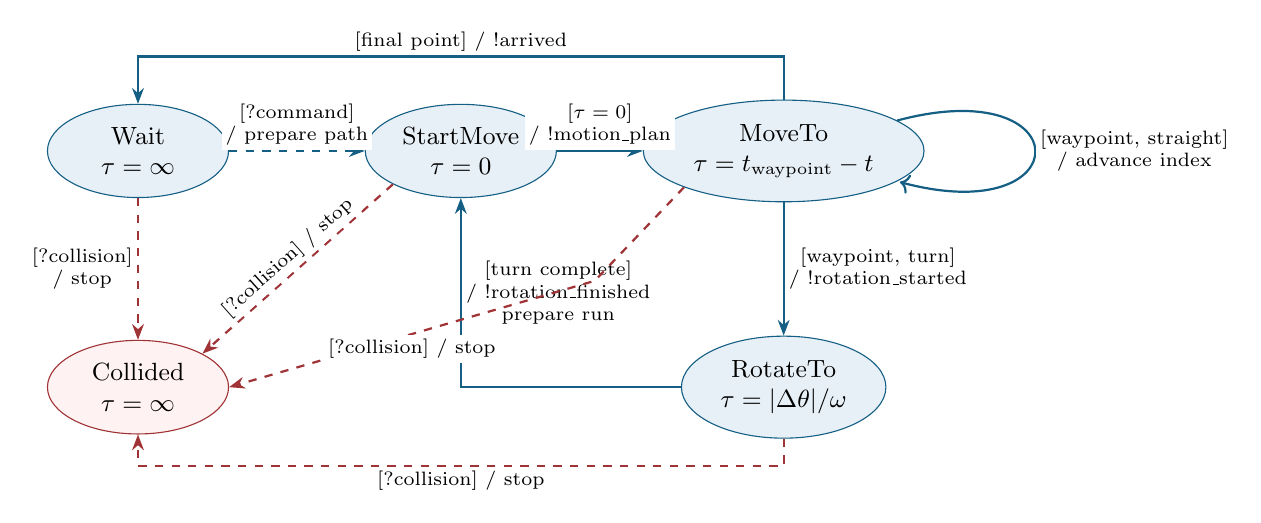
\begin{tikzpicture}[x=1cm,y=1cm]
\node[phase] (w) at (0,3) {Wait\\$\tau=\infty$};
\node[phase] (s) at (4.1,3) {StartMove\\$\tau=0$};
\node[phase] (m) at (8.2,3) {MoveTo\\$\tau=t_{\rm waypoint}-t$};
\node[phase] (r) at (8.2,0) {RotateTo\\$\tau=|\Delta\theta|/\omega$};
\node[terminal] (c) at (0,0) {Collided\\$\tau=\infty$};
\draw[ext] (w)--node[lab,above]{[?command]\\ / prepare path}(s);
\draw[flow] (s)--node[lab,above]{[$\tau=0$]\\ / !motion\_plan}(m);
\draw[flow] (m) edge[loop right] node[lab,right]{[waypoint, straight]\\ / advance index}(m);
\draw[flow] (m)--node[lab,right]{[waypoint, turn]\\ / !rotation\_started}(r);
\draw[flow] (r.west)--(4.1,0) -- node[lab,right]{[turn complete]\\ / !rotation\_finished\\prepare run}(s.south);
\draw[flow] (m.north)--(8.2,4.2)--node[lab,above]{[final point] / !arrived}(0,4.2)--(w.north);
\draw[crash] (w.south)--node[lab,left]{[?collision]\\ / stop}(c.north);
\draw[crash] (s.south west)--node[lab,above,sloped]{[?collision] / stop}(c.north east);
\draw[crash] (m.south west)--(5.8,1.35)--node[lab,below]{[?collision] / stop}(c.east);
\draw[crash] (r.south)--(8.2,-1)--node[lab,below]{[?collision] / stop}(0,-1)--(c.south);
\end{tikzpicture}}
\newcommand{\PSensorDiagram}{%
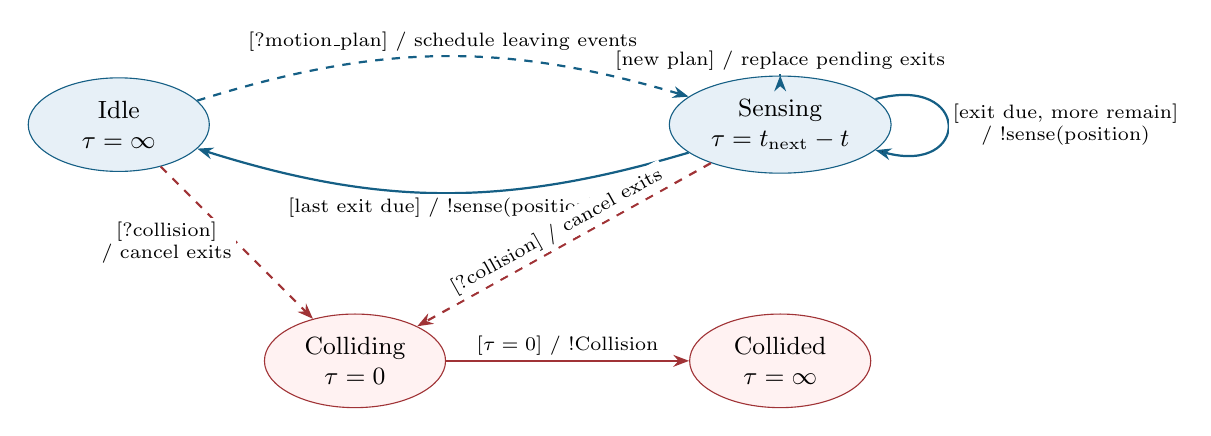
\begin{tikzpicture}[x=1cm,y=1cm]
\node[phase] (i) at (0,3) {Idle\\$\tau=\infty$};
\node[phase] (s) at (8.4,3) {Sensing\\$\tau=t_{\rm next}-t$};
\node[terminal] (g) at (3,0) {Colliding\\$\tau=0$};
\node[terminal] (c) at (8.4,0) {Collided\\$\tau=\infty$};
\draw[ext] (i) to[bend left=17] node[lab,above]{[?motion\_plan] / schedule leaving events}(s);
\draw[flow] (s) to[bend left=17] node[lab,below]{[last exit due] / !sense(position)}(i);
\draw[flow] (s) edge[loop right,looseness=5] node[lab,right]{[exit due, more remain]\\ / !sense(position)}(s);
\draw[ext] (s.north) to[out=120,in=60,looseness=3] node[lab,above]{[new plan] / replace pending exits}(s.north);
\draw[crash] (i)--node[lab,left]{[?collision]\\ / cancel exits}(g);
\draw[crash] (s)--node[lab,sloped,above]{[?collision] / cancel exits}(g);
\draw[flow,draw=collision] (g)--node[lab,above]{[$\tau=0$] / !Collision}(c);
\end{tikzpicture}}
\newcommand{\Profiles}{%
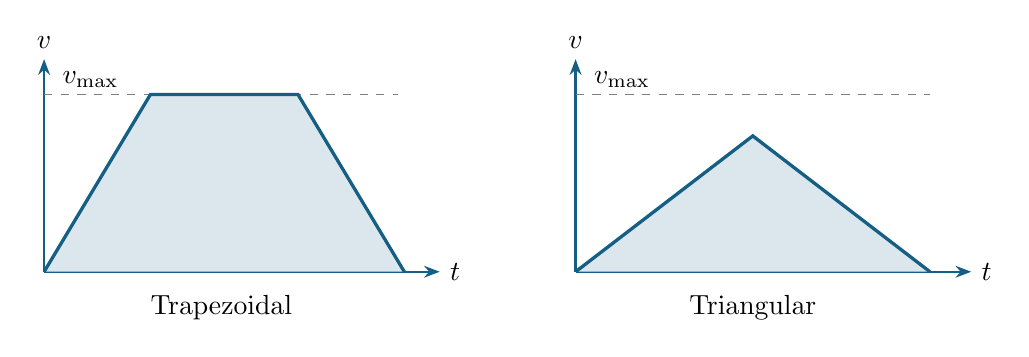
\begin{tikzpicture}[x=0.75cm,y=0.75cm]
\foreach \x in {0,9}{
 \draw[flow] (\x,0)--++(6.7,0) node[right] {$t$};
 \draw[flow] (\x,0)--++(0,3.6) node[above] {$v$};
 \draw[dashed,gray] (\x,3)--++(6,0);
}
\fill[accent!15] (0,0)--(1.8,3)--(4.3,3)--(6.1,0)--cycle;
\draw[accent,very thick] (0,0)--(1.8,3)--(4.3,3)--(6.1,0);
\fill[accent!15] (9,0)--(12,2.3)--(15,0)--cycle;
\draw[accent,very thick] (9,0)--(12,2.3)--(15,0);
\node at (3,-.6) {Trapezoidal};
\node at (12,-.6) {Triangular};
\node[anchor=west] at (.15,3.25) {$v_{\max}$};
\node[anchor=west] at (9.15,3.25) {$v_{\max}$};
\end{tikzpicture}}
\newcommand{\shot}[1]{\includegraphics[width=\linewidth,height=5.65cm,keepaspectratio]{assets/#1.png}}


\title{RMFS Implementation Design}
\setbeamertemplate{footline}{\hfill\scriptsize\color{accent}RMFS Implementation\quad\insertframenumber\ /\ \inserttotalframenumber\hspace{5mm}\vspace{3mm}}
\date{2026-11-19}
\begin{document}

\begin{frame}{RMFS 구현 설계: 자료 구조와 검증 기록}
\large 주어진 경로에서 분스복으로 무간섭 실행을 구성하기 위한 자료 구조
\par\bigskip\normalsize
이 문서는 이론 문서와 별도로 구현 결정을 기록한다.
현재 범위는 \textbf{자료 구조와 독립적인 분스복 검증 구현}이다.
뒤의 구현·검증 기록은 이 설계에 따른 첫 구현의 범위를 명시한다.
\par\bigskip
\begin{itemize}
\item 원 경로의 기하와 진행 순서를 보존한다.
\item 이동 부분경로와 점경로를 같은 구간 표현으로 다룬다.
\item 분스복은 원 경로 변경이 아니라 실행 순서열에 대기를 추가하는 연산이다.
\item 효율화와 분스합 탐색은 이후에 다룬다.
\end{itemize}
\par\medskip\small
책임 경계: RobotPathPlanner는 원 경로 생성, TrafficManager는 교통 제어를 담당한다.
검증은 작은 독립 객체에서 먼저 진행하고, 이후 TrafficManager의 재사용 또는 이식을 검토한다.
TrafficManager에는 아직 통합하지 않는다. 검증용 일반 객체의 API는 뒤에 기록한다.
\end{frame}

\begin{frame}{자료 구조의 관계}
\begin{center}\begin{tikzpicture}[node distance=12mm]
\node[module] (p) at (0,2.5) {Path\\원 경로};
\node[module] (u) at (0,.5) {Subpath\\원 경로 구간 참조};
\node[module] (s) at (4,.5) {Sweep\\파생 점유 영역};
\node[module] (c) at (4,2.5) {InterferenceSet\\경로상 간섭 구간};
\node[module] (t) at (-4,.5) {TuplePath\\묶음의 순서열};
\draw[flow] (u)--node[lab,left]{참조}(p);
\draw[flow] (u)--(s);
\draw[flow] (s)--node[lab,right]{상대 스윕과 비교}(c);
\draw[flow] (t)--(u);
\end{tikzpicture}\end{center}
\small 화살표는 참조 또는 계산 관계이며 DEVS coupling이 아니다.
Path는 원 자료이고, Subpath는 경로 일부를 지정한다.
Sweep은 점유 영역이며, InterferenceSet은 그 영역 자체가 아니라 원 경로에서 간섭하는 위치를 기록한다.
TuplePath는 각 물체의 이동과 대기를 공통 단계로 맞춘 실행 표현이다.
\end{frame}

\begin{frame}{원 경로와 경로상의 위치}
\footnotesize
\begin{tabular}{p{2.5cm}p{4.2cm}p{5.6cm}}\toprule
자료 & 내용 & 규칙\\\midrule
Path & 경로 식별자, 순서 있는 정점 벡터 배열 & 각 정점은 $n$차원 부동소수점 벡터다. 한 경로의 차원은 동일하며, 원 경로는 실행 중 변경하지 않는다.\\
PathPosition & 경로상의 진행 위치 & 공간 좌표와 구별한다. 서로 다른 경로의 진행 위치를 직접 비교하지 않는다.\\
Subpath & Path 참조, 시작·끝 진행 위치 & 시작은 끝보다 뒤에 올 수 없다. 양 끝이 같으면 점경로다.\\\bottomrule
\end{tabular}
\par\medskip
정점 $p_k=(x_{k,1},\ldots,x_{k,n})\in\mathbb R^n$의 각 성분은 부동소수점 수다.
현재 RMFS 예제는 $n=2$이며 위치 좌표의 단위는 m다.
\par\smallskip
지정한 점 $p_k$의 진행 위치는 정수 $k$로 표현한다. 선분 내부까지 필요하면
$k+\lambda$ ($0\le\lambda<1$)에 해당하는 $(k,\lambda)$ 표현을 사용한다.
마지막 점은 $(m,0)$으로 표현한다. 정점의 표현을 하나로 정규화한다.
\[
 (k,\lambda)\longmapsto (1-\lambda)p_k+\lambda p_{k+1}.
\]
\textbf{기하 경계와 실행 경계의 구별:}
간섭은 선분 내부에서 시작할 수 있다. 그러나 초기 분스복 실험에서는
실행 부분경로의 양 끝을 주어진 유한한 점에 한정한다.
간섭 경계를 계산했다고 임의의 새 정지점을 허용하는 것은 아니다.
\par\medskip\footnotesize
물체별 경로 배정과 축 정렬 점유 사각형의 크기는 별도 입력이다.
초기 방향과 운동 파라미터는 물리 실행에 필요하며, 경로 좌표나 대기 복사와 혼합하지 않는다.
\end{frame}

\begin{frame}{스윕과 간섭집합}
\small
\begin{tabular}{p{2.5cm}p{4.2cm}p{5.6cm}}\toprule
자료 & 내용 & 규칙\\\midrule
Sweep & 차원과 영역들의 배열 & 각 영역은 차원 및 교차 검사 기능을 갖는다. 전체는 이 영역들의 합집합이다.\\
InterferenceSet & Path 참조와 진행 구간들의 순서열 & 경로 진행 순으로 정렬하고 겹치거나 맞닿은 구간을 합친다. 빈 집합을 허용한다.\\\bottomrule
\end{tabular}
\par\medskip
\textbf{현재 2D RMFS에서의 계산:} 일반 Sweep의 영역을 축 정렬 직사각형으로 구현한다.
이는 2차원 특수화다. 고정된 축 정렬 사각형이 수평·수직 선분을 이동하면
그 스윕은 직사각형이다. 점경로의 스윕도 물체 크기의 사각형이다.
여러 직사각형의 겹침은 허용하며 전체 스윕은 그 합집합으로 해석한다.
\par\medskip
\textbf{간섭집합의 의미:} 물체 $i$의 경로에서 상대의 전체 스윕과
자기 점유 영역이 교차하는 진행 구간을 기록한다.
복수 물체에 대해서는 지정한 모든 상대에 대한 구간의 합집합을 사용한다.
비교 대상 물체 집합도 결과와 함께 식별할 수 있어야 한다.
\par\medskip
\textbf{경계 규칙 제안:} 사각형 경계가 닿는 경우도 간섭으로 판정한다.
부동소수점 허용오차와 별도의 물리 안전 여유는 독립된 인자로 받는다.
\par\smallskip\footnotesize
Sweep은 Subpath와 점유 크기에서 계산하는 파생 자료다.
캐시는 정확성 확인 후 필요할 때 도입한다. 경로 인덱스만으로 스윕을 식별하면
물체 크기가 다른 경우를 구별할 수 없으므로 주의한다.
\end{frame}

\begin{frame}{묶음 경로와 분스복의 표현}
\small
물체 순서를 고정하고, 각 단계의 묶음을 물체별 Subpath 참조의 튜플로 둔다.
TuplePath는 이 묶음들의 순서열이다. 두 물체일 때는 짝 경로다.
\[
 \mathcal P=\bigl((P_{1,k},\ldots,P_{n,k})\bigr)_{k=1}^{M}.
\]
\begin{center}\begin{tikzpicture}[x=1cm,y=.8cm]
\node[left] at (0,1){물체 1};\node[left] at (0,0){물체 2};
\node[draw,minimum width=4cm] at (2.3,1){시작 점경로의 복사};
\node[draw,minimum width=4cm] at (7.3,1){원 경로의 이동};
\node[draw,minimum width=4cm] at (2.3,0){원 경로의 이동};
\node[draw,minimum width=4cm] at (7.3,0){종점경로의 복사};
\draw[dashed] (4.8,-.5)--(4.8,1.5);
\end{tikzpicture}\end{center}
\textbf{복사할 자료:} 동일한 점경로 참조를 실행 순서열에 다시 삽입한다.
원 좌표 배열이나 물리 물체를 복제하지 않는다.
\par\medskip
\textbf{검사할 불변조건:}
각 물체의 성분은 시작부터 종점까지 원래 순서로 이어지고,
추가된 항목은 점경로 대기다. 각 묶음에서 모든 성분 쌍의 스윕이 무간섭이어야 한다.
현재 묶음을 모두 완료한 후 다음 묶음을 시작한다.
\par\medskip\footnotesize
이 표현은 실행 순서를 기록하며 수치적인 대기시간은 아직 저장하지 않는다.
물리 실행에서는 먼저 도착한 물체가 나머지 성분의 완료까지 끝점에서 기다린다.
\end{frame}

\begin{frame}{합의한 구현 범위와 검증 순서}
\small
\begin{tabular}{p{.7cm}p{5cm}p{6.7cm}}\toprule
번호 & 검토 항목 & 현재 상태\\\midrule
1 & 진행 위치의 타입과 정규화 & 정수 정점 + 선분 내부 비율; 비율 1은 다음 정점으로 정규화\\
2 & 수치 허용오차와 안전 여유 & 각각 독립 인자; 기본값 $10^{-9}$ m, 0 m\\
3 & 실행 부분경로의 경계 & 주어진 유한한 정점에서만 이동 시작·종료·대기\\
4 & 테스트용 객체와 통합 범위 & WaitDuplicationSolver; DEVS·TrafficManager 변경 없음\\\bottomrule
\end{tabular}
\par\bigskip
\textbf{검증 순서:}
부분경로·점경로 표현 $\to$ 스윕 계산 $\to$ 간섭집합 계산
$\to$ 분스복으로 만든 묶음 경로의 무간섭·전체 완료 검사.
\par\medskip
먼저 작은 예제로 계산 결과를 직접 확인한다. 이후 해가 있는 경우와 없는 경우를
모두 포함해 분스복 탐색을 검증한다. 애니메이션 연결은 자료와 계산의 검증 이후에 진행한다.
\par\bigskip
이 문서는 구현 검토와 검증 기록이며, 이론 문서의 정리와 증명을 대체하지 않는다.
\end{frame}

\begin{frame}{첫 구현: 자료 구조와 공개 함수}
\small
\texttt{examples/RMFS/path\_geometry.py}는 DEVS·Viewer와 독립적이다.
\begin{itemize}
\item Path, PathPosition, Subpath: $n$차원 정점과 정규화한 경로상의 위치.
\item Sweep, Region: 차원에 독립적인 합집합 표현과 영역 교차 인터페이스.
\item AABB: 차원 일반적인 축 정렬 상자. 현재 스윕 계산기는 2D만 제공한다.
\item \texttt{sweep\_2d}: 부분경로와 점유 크기에서 직사각형 스윕 계산.
\item \texttt{interference\_2d}: 선분과 확장된 상대 스윕의 구간 교차를 해석적으로 계산.
고정 시간 간격의 샘플링은 사용하지 않는다.
\item InterferenceSet: 구간 정렬·합체, 시작·종 경계 및 유한한 점에서 확장 경계 선택.
\item TuplePath: 모든 성분을 명시한 [단계][물체] 배열. 희소 표현은 사용하지 않는다.
\end{itemize}
\par\medskip
경계 접촉은 간섭이다. 허용오차는 간격 비교를 보수적으로 확장하고,
안전 여유는 각 물체의 점유 사각형을 각 방향으로 팽창시킨다.
기본값은 각각 $10^{-9}$ m와 0 m다. 물체별 서로 다른 크기도 입력 가능하다.
\end{frame}

\begin{frame}{분스복 탐색: 유한 상태의 완전 탐색}
\small
\texttt{examples/RMFS/wait\_duplication.py}의 WaitDuplicationSolver는 일반 객체다.
원 경로의 구성열은 $p_0,e_{01},p_1,\ldots,p_m$이며 분스합을 하지 않는다.
상태는 각 물체가 소비한 원 구성 항목 수 $(k_1,\ldots,k_n)$다.
\par\medskip
각 물체는 다음 원 항목 하나를 실행하거나 현재 점경로를 복사해 대기한다.
모든 물체 쌍의 스윕이 무간섭인 묶음만 허용한다.
전원 대기는 상태를 바꾸지 않으므로 제외한다.
\par\medskip
\textbf{API:} \texttt{solve()}는 feasible 또는 infeasible을 반환한다.
성공 결과에는 TuplePath와 구성 항목 소비 기록을 포함한다.
\texttt{validate(result)}는 원 구성 순서·대기 복사·목표 도달·각 묶음의 교차를
스윕 캐시를 믿지 않고 다시 계산해 검사한다.
\par\medskip
너비 우선 탐색으로 모든 허용된 다음 묶음을 열거한다.
같은 진행 상태는 다시 확장하지 않는다. 상태 수는 최대
$\prod_i(r_i+1)$이며 $r_i$는 원 구성 항목 수다.
수치적 시간이나 이력 의존 자원이 없는 현재 모델에서는 진행 상태가 같으면
가능한 후속 실행도 같다. 따라서 방문 상태 제거로 해를 잃지 않는다.
\par\medskip\footnotesize
infeasible은 제한 시간 종료가 아니라 유한 탐색의 소진을 뜻한다.
판정 범위는 주어진 정점 분할과 무간섭 스윕 묶음이다.
정밀한 시간차만으로 스쳐 통과하는 해, 임의의 새 정지점, 우회·후진은 탐색하지 않는다.
\end{frame}

\begin{frame}{기존 두 물체 예제 검증: 11개}
\small\renewcommand{\arraystretch}{1.12}
\begin{tabular}{p{1.1cm}p{5.8cm}p{2cm}rr}\toprule
예제 & 이름 & 판정 & 묶음 수 & 방문 상태\\\midrule
02\_01 & Crossing NoControl & 해 있음 & 10 & 60\\
02\_02 & LeftEdge NoControl & 해 있음 & 7 & 60\\
02\_03 & SameDirection Collision & 해 있음 & 11 & 88\\
02\_04 & SameDirection Clear & 해 있음 & 11 & 44\\
02\_05 & OppositeDirection Collision & 해 없음 & -- & 24\\
02\_06 & OppositeDirection Clear & 해 있음 & 11 & 52\\
02\_07 & OppositeDirection EntryWait & 해 있음 & 20 & 104\\
02\_08 & DisjointSweeps & 해 있음 & 7 & 64\\
02\_09 & FirstMoverMatters & 해 있음 & 8 & 36\\
02\_10 & AlternatingProgress & 해 있음 & 11 & 128\\
02\_11 & SharedCorner & 해 있음 & 26 & 196\\\bottomrule
\end{tabular}
\par\medskip\footnotesize
기존 예제의 원 경로를 그대로 사용했다. 원 예제의 이름에 Collision이 있어도
분스복을 넣은 경로에는 해가 있을 수 있다. 점경로 항목도 단계로 세므로 묶음 수는
물리적 이동 횟수나 makespan이 아니다. 기존 무제어 애니메이션은 변경하지 않았다.
\end{frame}

\begin{frame}{기존 세 물체 예제 검증: 6개}
\small\renewcommand{\arraystretch}{1.2}
\begin{tabular}{p{1.1cm}p{5.8cm}p{2cm}rr}\toprule
예제 & 이름 & 판정 & 묶음 수 & 방문 상태\\\midrule
03\_01 & ThreeWay Collision & 해 없음 & -- & 56\\
03\_02 & ThreeFollowing Collision & 해 있음 & 15 & 1344\\
03\_03 & MixedDirection Collision & 해 없음 & -- & 80\\
03\_04 & SweepInterference & 해 있음 & 11 & 976\\
03\_05 & LocalSafe Deadlock & 해 있음 & 20 & 416\\
03\_06 & ThreeWay CyclicWait & 해 없음 & -- & 32\\\bottomrule
\end{tabular}
\par\bigskip
\textbf{합계:} 기존 17개 중 13개는 무간섭 묶음 경로를 구성했고,
4개는 전체 탐색을 소진하여 해 없음으로 판정했다.
\par\medskip
03\_05는 안전한 이동을 잘못 선택하면 막히는 예제다.
전체 탐색에서는 다른 선택을 통해 완료하는 경로를 찾는다.
따라서 국소적으로 막힌 상태와 초기 문제 자체의 불가능성을 구별한다.
\par\medskip\footnotesize
2 m 격자, 모든 물체의 점유 크기 $1.5\times1.5$ m,
허용오차 $10^{-9}$ m, 안전 여유 0 m를 사용했다.
실행 속도·회전시간·PSensor 이벤트는 이번 기하 검증의 대상이 아니다.
\end{frame}

\begin{frame}{검증 근거와 재실행}
\small
\textbf{30개 테스트 통과.} 경계 접촉, 수치 오차와 안전 여유, 선분 내부의 정확한
간섭 경계, 분리된 간섭구간, 3D 정점 표현, 2D 전용 계산기의 차원 검사,
정지·완료 물체의 점유, 서로 다른 물체 크기 및 잘못된 실행 기록 거부를 확인했다.
\par\medskip
\textbf{독립 기준 계산과 비교.} 생산 코드의 스윕·교차·후속 상태 함수를 호출하지 않는
별도 정점 진행 DAG 계산기로 기존 17개와 작은 격자의 방향성 선분 쌍 64개를 검사했다.
모든 해 유무 판정이 일치했다. 성공 결과는 원래 점경로 항목까지 포함해 재검사했다.
\par\medskip
\textbf{실행 명령:}\par\smallskip
{\scriptsize\ttfamily python -m examples.RMFS.Tests.run\_wait\_duplication}\par
{\scriptsize\ttfamily python -m pytest tests/examples/RMFS/test\_wait\_duplication.py -q}
\par\medskip
\textbf{결과 파일:}\par
{\scriptsize\ttfamily examples/RMFS/Tests/results/wait\_duplication\_examples.json}
\par\medskip\footnotesize
JSON에는 각 예제의 판정·탐색 통계·간섭구간·성공 묶음·진행 기록을 저장했다.
별도 실행은 \texttt{--output} 인자로 결과 파일을 지정한다.
이 검증은 분스복 구현의 회귀 검사이며, 모든 물리 상황의 충돌 회피를 실험으로 증명했다는 뜻은 아니다.
\end{frame}

\end{document}
